\documentclass [a4paper]{article}
\title{Mini-Projet}
\author{GUO Lieqiang}
\usepackage{Sweave}
\begin{document}
\Sconcordance{concordance:test-sweave.tex:test-sweave.Rnw:%
1 3 1 1 0 4 1 1 2 1 0 2 1 8 0 1 1 6 0 1 2 2 1 1 2 4 1 1 -13 1 0 2 1 8 0 %
1 1 9 0 1 15 1 1 1 2 1 0 1 1 5 0 5 1 7 0 6 1 1 4 3 0 2 1 5 0 1 1 1 2 2 %
1 1 4 3 0 2 1 5 0 1 1 4 0 1 2 2 1 2 2 1 1}

\maketitle
In this example we embed parts of the examples from the
\texttt {kruskal.test} help page into a \LaTeX{}document:
\begin{Schunk}
\begin{Sinput}
> data(airquality , package ="datasets")
> library ("stats")
> kruskal.test(Ozone ~ Month , data = airquality)
\end{Sinput}
\begin{Soutput}
	Kruskal-Wallis rank sum test

data:  Ozone by Month
Kruskal-Wallis chi-squared = 29.2666, df = 4, p-value = 6.901e-06
\end{Soutput}
\begin{Sinput}
> 1+4
\end{Sinput}
\begin{Soutput}
[1] 5
\end{Soutput}
\end{Schunk}
which shows that the location parameter of the Ozone
distribution varies significantly from month to month . Finally we
include a boxplot of the data :
$
\begin{}
{44}
\end{}
$
\begin{Schunk}
\begin{Sinput}
> data(airquality , package ="datasets")
> library ("stats")
> kruskal.test(Ozone ~ Month , data = airquality)
\end{Sinput}
\begin{Soutput}
	Kruskal-Wallis rank sum test

data:  Ozone by Month
Kruskal-Wallis chi-squared = 29.2666, df = 4, p-value = 6.901e-06
\end{Soutput}
\begin{Sinput}
> 1+4
\end{Sinput}
\begin{Soutput}
[1] 5
\end{Soutput}
\begin{Sinput}
>   
\end{Sinput}
\end{Schunk}

\begin{center}
\begin{Schunk}
\begin{Sinput}
> library("graphics")
> 1+2
\end{Sinput}
\begin{Soutput}
[1] 3
\end{Soutput}
\begin{Sinput}
> a <- 5/100;
> n <- c(10, 100, 1000);
> quantille <- 1-a/2;
> A_n <- qnorm(quantille)/sqrt(n);
> t(matrix(c(n,A_n),3))
\end{Sinput}
\begin{Soutput}
          [,1]        [,2]        [,3]
[1,] 10.000000 100.0000000 1.00000e+03
[2,]  0.619795   0.1959964 6.19795e-02
\end{Soutput}
\begin{Sinput}
> u <- 0.1;
> n0 <- 0;
> R_H1 <- c();
> beta <- 0.95;
> n <- seq(50,5000,200);
> A_n <- qnorm(quantille)/sqrt(n)
> for (i in n){
+   temp_R_H1 <- pnorm(q = A_n[which(i==n)], mean = u, sd = sqrt(1/i)) - pnorm(q = - A_n[which(i==n)], mean = u, sd = sqrt(1/i))
+   R_H1 <- c(R_H1, temp_R_H1)
+ }
> n0 <- n[min(which((1 - R_H1) >= beta))]
> n0
\end{Sinput}
\begin{Soutput}
[1] 1450
\end{Soutput}
\begin{Sinput}
> plot(n, R_H1, type = 'l')
> n <- seq(50,n0,1)
> A_n <- qnorm(quantille)/sqrt(n)
> R_H1 <- c()
> for (i in n){
+   temp_R_H1 <- pnorm(q = A_n[which(i==n)], mean = u, sd = sqrt(1/i)) - pnorm(q = - A_n[which(i==n)], mean = u, sd = sqrt(1/i))
+   R_H1 <- c(R_H1, temp_R_H1)
+ }
> n0 <- n[min(which((1 - R_H1) >= beta))]
> n0
\end{Sinput}
\begin{Soutput}
[1] 1300
\end{Soutput}
\begin{Sinput}
> boxplot( Ozone ~ Month , data = airquality )
\end{Sinput}
\end{Schunk}
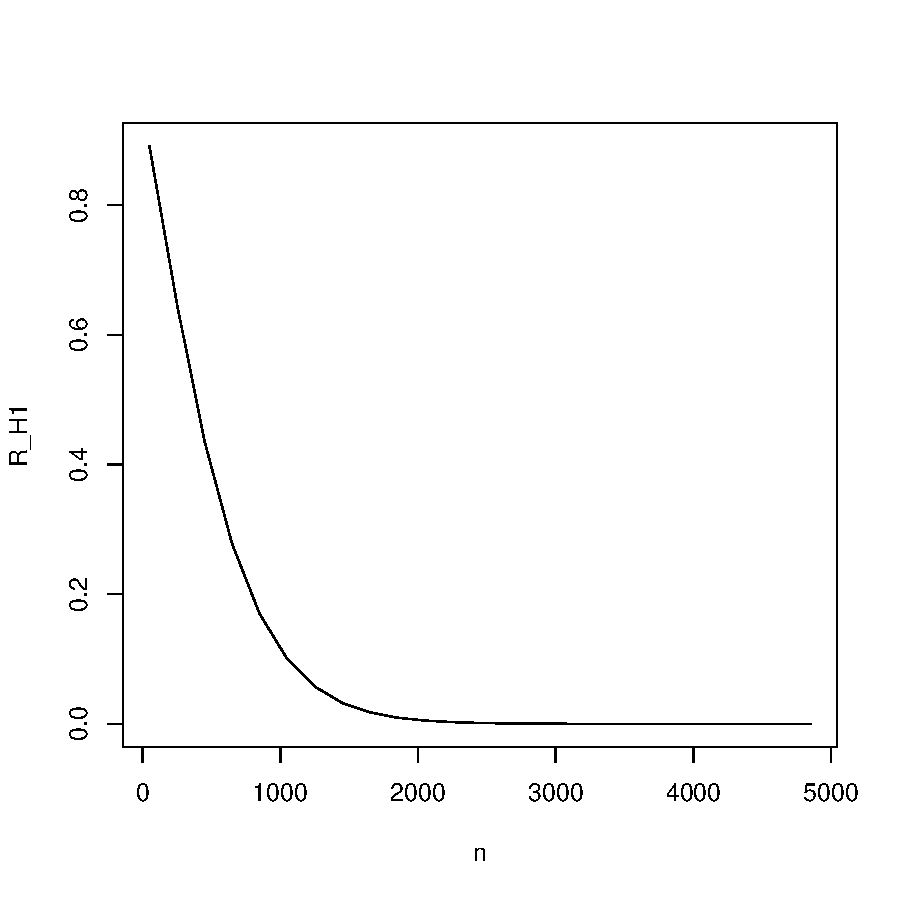
\includegraphics{test-sweave-003}

\end{center}
\begin{center}
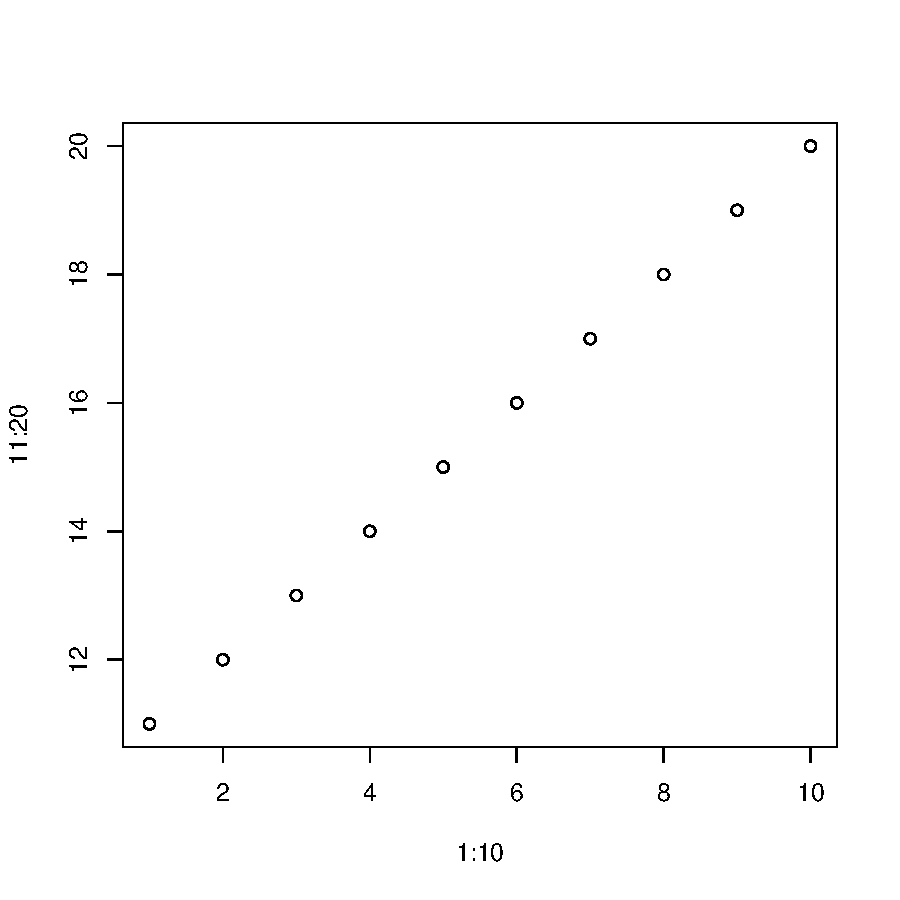
\includegraphics{test-sweave-004}
\end{center}
\end{document}
